\documentclass{article}
\usepackage[utf8]{inputenc}
\usepackage{amsmath}
\usepackage{listings}
\usepackage{geometry}
\usepackage{graphicx}
\usepackage{subfig}
\usepackage[colorlinks=true]{hyperref}
\title{%
Project 2 - Eigenvalue Problems \\
\large FYS3150 at University of Oslo}
\author{Simen Løken}
\date{September 2020}
\footskip = 90pt
\topmargin = -40pt

\begin{document}
\nocite{lec}
\maketitle
\section{Abstract}
In this project we'll show four ways to uniquely extract from a matrix it's respective eigenvalues and accompanying eigenvectors. Additionally we'll weigh these methods against each other to better find out which method is best suited for our purpose and why. \newline
We'll also be solving a harmonically oscillating one-dimensional one electron system numerically using a Jacobi rotation algorithm and find that it's eigenstates are given as $\lambda_1 = 3, \lambda_2 = 7, \lambda_3 = 11$.
\section{Introduction}
An eigenvector is a nonzero vector of a linear transformation that changes by a scalar factor when said linear transformation is applied. All eigenvectors have a corresponding eigenvalue, which is the eigenvectors' scaling factor.\newline 
Eigenvalues have a surprisingly wide range of uses. Oil companies will use linear systems to map out the ocean floor and then use those mappings' eigenvalues to give an indication of where you can find oil reserves. Eigenvalues have also found use in designing car stereo systems that help reproduce the vibration of the car due to the music. Additionally, eigenvalues have also found a use as a good indicator for how stable a bridge is. The natural frequency of a bridge is given as the smallest eigenvalue of the system that models that particular bridge \cite{artic}. This is a clue to what we're going to be looking at, the buckling beam problem, and might clue us in as to why we're coupling the buckling beam problem and eigenvalues in the same project.
\section{Theory and Method}
In this project we'll be using Jacobi's method to diagonalize our matrices. Jacobi's method means we'll be performing rotations in our hyperplanes to zero out diagonal elements. \newline
To justify using this method, we'll have to show that Jacobi's method retains the dot product and the orthogonality. \newline
Let's assume we rotate a vector $\Vec{v}$ with a matrix \textbf{U} such that:
\begin{equation*}
    \Vec{v}_i \xrightarrow[]{} \Vec{v}_i' = \textbf{U}^T \Vec{v}_i
\end{equation*} \newpage
It then follows that are matrix operations are:
\begin{equation*}
    \textbf{A} \xrightarrow[]{} \textbf{A}' = \textbf{U}^T \textbf{A} \textbf{U}
\end{equation*}
If we can now show that such a transformation of our vector $\Vec{v}_i$ retains orthogonality and dot product, this method is valid. Remind yourself that:
\begin{equation*}
    v_{j}^{T}v_i = \delta_{ij}
\end{equation*}
And as such, we can check:
$$\Vec{v}_i'\cdot \Vec{v}_j' = \Vec{v}_i^{T}' \Vec{v}_j'$$
$$\Vec{v}_i'\cdot \Vec{v}_j' = (\textbf{U}^T \Vec{v}_i)^T \textbf{U}^T \Vec{v}_j $$
$$\Vec{v}_i'\cdot \Vec{v}_j' = \Vec{v}_i^T \textbf{U}\textbf{U}^T \Vec{v}_j$$
$$\Vec{v}_i'\cdot \Vec{v}_j' = \Vec{v}_i^T \Vec{v}_j$$
$$\Vec{v}_i'\cdot \Vec{v}_j' = \Vec{v}_i \cdot \Vec{v}_j$$
We see that our right-hand side is the dot-product from before our transformation, and as such we can conclude that the dot product and orthogonality has been retained.
\newline
As our orthogonality and dot products are retained, we can, in theory, calculate the eigenvalues of a given matrix by
\begin{equation} \label{1}
    -\frac{u(\rho_i+h) -2u(\rho_i) +u(\rho_i-h)}{h^2}  = \lambda u(\rho_i)
\end{equation}
\newline
where $\rho_i = \rho_0 + ih$ and $h$ is the step-size \newline
This is, in practice, a tridiagonal matrix given as:
\begin{equation}
    \begin{bmatrix} d& a & 0   & 0    & \dots  &0     & 0 \\
                                a & d & a & 0    & \dots  &0     &0 \\
                                0   & a & d & a  &0       &\dots & 0\\
                                \dots  & \dots & \dots & \dots  &\dots      &\dots & \dots\\
                                0   & \dots & \dots & \dots  &a  &d & a\\
                                0   & \dots & \dots & \dots  &\dots       &a & d\end{bmatrix} 
                                 \begin{bmatrix} u_1 \\ u_2 \\ u_3 \\ \dots \\ u_{N-2} \\ u_{N-1}\end{bmatrix} = \lambda \begin{bmatrix} u_1 \\ u_2 \\ u_3 \\ \dots \\ u_{N-2} \\ u_{N-1}\end{bmatrix} . 
\label{eq:matrixse} 
\end{equation}
This relation has been shown in Project 1 \cite{proj1}
Eigenvalues are then analytically given as
\begin{equation}
    \lambda_j = d+2a\cos{(\frac{j\pi}{N})}, \hspace{0.2cm} j=1,2,\dots N-1.
\end{equation}
\newline
Now, to use Jacobi's Rotation Algorithm we'll need to define $\tan \theta$.
\begin{equation*}
    \tan \theta = \frac{\sin \theta}{\cos \theta} = \frac{s}{c}
\end{equation*}
\newpage
This can be rewritten as:
\begin{equation*}
    \cot 2\theta=\tau = \frac{a_{ll}-a_{kk}}{2a_{kl}}
\end{equation*}
\newline
where $a_{ll}$ and $a_{kk}$ are matrix elements given by the coordinates $[l,l]$ and $[k,k]$, respectively. \newline
We can then define our angle $\theta$ so that our non-diagonal matrix elements become non-zero. \newline
We then get the quadratic equation:
\begin{equation*}
    t^2+2\tau t-1= 0,
\end{equation*}
\newline giving us
\begin{equation*}
  t = -\tau \pm \sqrt{1+\tau^2},
\end{equation*}
\newline
$c$ is then given as:
\begin{equation}
    c = \frac{1}{\sqrt{1+t^2}}
\end{equation}
and s as:
\begin{equation}
    s = tc
\end{equation}
We can then use the following code-block to rotate our matrix and get the eigenvalues:
\begin{lstlisting}[language=Python]
for i in range(n):
        kvec = vec[i,k]
        lvec = vec[i,l]
        vec[i,k] = c*kvec - s*lvec
        vec[i,l] = c*lvec + s*kvec
        if i not in [k, l]:
            kmat = mat[i,k]; lmat = mat[i,l]
            mat[i,k] = c*kmat - s*lmat
            mat[i,l] = c*lmat + s*kmat
            mat[k,i] = mat[i,k]
            mat[l,i] = mat[i,l]
\end{lstlisting} \newline
We'll also be expanding upon our previously derived model to include quantum mechanics. \newline
Primarily we're interested in including a one dimensional potential $V(r)$ to our matrix. The TISE (Time Independent Schrödinger Equation in it's radial form is given as
\begin{equation}
    -\frac{\hbar^2}{2 m} \left ( \frac{1}{r^2} \frac{d}{dr} r^2
  \frac{d}{dr} - \frac{l (l + 1)}{r^2} \right )R(r) 
     + V(r) R(r) = E R(r).
\end{equation}
It's energy states are then given as:
\begin{equation}
    E_{nl}=  \hbar \omega \left(2n+l+\frac{3}{2}\right)
\end{equation}
Since we're using spherical coordinates we can substitute R(r) = $\frac{1}{r}$ u(r) and obtain:
\begin{equation*}
  -\frac{\hbar^2}{2 m} \frac{d^2}{dr^2} u(r) 
       + \left ( V(r) + \frac{l (l + 1)}{r^2}\frac{\hbar^2}{2 m}
                                    \right ) u(r)  = E u(r) .
\end{equation*}
\newline
If we now introduce a dimensionless variable $\rho = r\frac{1}{\alpha}$, we can set $l = 0$ and insert for $V(\rho$ and get:
\begin{equation*}
  -\frac{d^2}{d\rho^2} u(\rho) 
       + \frac{mk}{\hbar^2} \alpha^4\rho^2u(\rho)  = \frac{2m\alpha^2}{\hbar^2}E u(\rho) .
\end{equation*}
We can now rewrite our Schrödinger equation as:
\begin{equation}
  -\frac{d^2}{d\rho^2} u(\rho) + \rho^2u(\rho)  = \lambda u(\rho) .
\end{equation}
\newline
This looks pretty similar to our Equation [\ref{1}], and we can write
\begin{equation}
    -\frac{u(\rho_i+h) -2u(\rho_i) +u(\rho_i-h)}{h^2}+\rho_i^2u(\rho_i)  = \lambda u(\rho_i)
\end{equation}
In this system, we define our diagonal and sub-diagonal matrix element to be:
\begin{equation}
   d_i=\frac{2}{h^2}+V_i,
\end{equation}
\begin{equation}
   e_i=-\frac{1}{h^2}.
\end{equation}
Such that we get the matrix system:
\begin{equation*}
    \begin{bmatrix}d_1 & e_1 & 0   & 0    & \dots  &0     & 0 \\
                                e_1 & d_2 & e_2 & 0    & \dots  &0     &0 \\
                                0   & e_2 & d_3 & e_3  &0       &\dots & 0\\
                                \dots  & \dots & \dots & \dots  &\dots      &\dots & \dots\\
                                0   & \dots & \dots & \dots  &\dots  e_{N-3}     &d_{N-2} & e_{N-2}\\
                                0   & \dots & \dots & \dots  &\dots       &e_{N-2} & d_{N-1}
             \end{bmatrix}  \begin{bmatrix} u_{1} \\
                                                              u_{2} \\
                                                              \dots\\ \dots\\ \dots\\
                                                              u_{N-1}
             \end{bmatrix}=\lambda \begin{bmatrix} u_{1} \\
                                                              u_{2} \\
                                                              \dots\\ \dots\\ \dots\\
                                                              u_{N-1}
             \end{bmatrix}.  
      \label{eq:sematrix}
\end{equation*}
We can then use our Jacobi Rotation Algorithm to solve this system with the same code as shown above. For a more complete derivation of of this matrix system and the radial Scrödinger Equation, see \cite{projText}
\newline
Lastly we'll be looking at an alternative method of finding the eigenvalues of a tridiagonal matrix.
For simplicity's sake, assume we have a matrix $\mathbf{A}$:
\[
\mathbf{A} = 
\begin{bmatrix} d& a & 0   & 0    & \dots  &0     & 0 \\
                                a & d & a & 0    & \dots  &0     &0 \\
                                0   & a & d & a  &0       &\dots & 0\\
                                \dots  & \dots & \dots & \dots  &\dots      &\dots & \dots\\
                                0   & \dots & \dots & \dots  &a  &d & a\\
                                0   & \dots & \dots & \dots  &\dots       &a & d\end{bmatrix} 
\] \newline
We know that in order to find the eigenvalues we can find the characteristic polynomial of the matrix and find it's roots. \newpage
One simple way of finding these roots is to employ the bisection method. 
Assume we're looking for a root of a function $f(x)$ and that we know that a root exists between $f(a)$ and $f(b)$, or rather, that our function crosses the x-axis. It then follows that the center between these points is given as:
\begin{equation*}
    c = \frac{a+b}{2}
\end{equation*} \newline
If $f(c)$ happens to be 0, or close to 0 within a tolerance, then we're close to a root, and can extract $c$ as a root of $f(x)$ \newline
In code, this is:
\begin{lstlisting}[language=Python]
def bisection(f,a,b,N):
    for n in range(1,N+1):
        c = (a + b)/2
        fc = f(c)
        if f(a)*fc < 0:
            a = a
            b = c
        elif f(b)*fc < 0:
            a = c
            b = b
        elif fc == 0:
            return c
        else:
            return None
    return (a + b)/2   
\end{lstlisting}
\newpage
\section{Results}
We ran our Jacobi Algorithm and found very similar results to the analytical and built-in numpy function. \newline For $n = 5, d = 5, a = 2$ we found:
\begin{table}[ht!]
    \centering
    \begin{tabular}{c|c|c}
         Analytical& Numpy& Jacobi& \\
         1.53589838& 1.53589838& 1.53589838& \\
         3& 3& 3& \\
         5& 5& 5& \\
         7& 7& 7& \\
         8.46410162& 8.46410162& 8.46410162& 
    \end{tabular}
    \caption{Eigenvalues given by the three different algorithms}
    \label{tab:my_label}
\end{table}
\newline
As such we have validated that our Jacobi method works correctly. A more interesting point would be computation speed. \newline
We let the algorithms run though the matrix $a = -5, d = 10$ but for different values of N.\newline We let N be $N = [5,10,30,50]$
This gives us the following plot:
\begin{figure}[ht!]
    \centering
    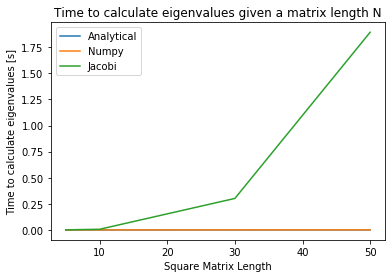
\includegraphics[scale=0.6]{figure2.png}
    \caption{Runtimes for the three algorithms, analytical, numpy and Jacobian respectively.}
    \label{fig:1}
\end{figure} \newline
An interesting take-away from this is that the Jacobi Algorithm is pretty slow all things considered, with runtimes increasing exponentially as N increases. \newpage As for the analytical and numpy solutions they look like this:
\begin{figure}[ht!]
    \centering
    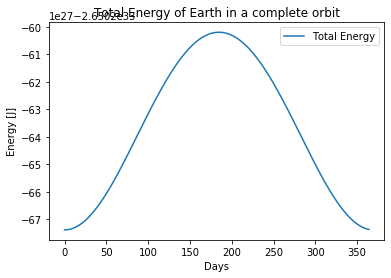
\includegraphics[scale=0.6]{figure4.png}
    \caption{A "zoomed in" view of the analytical and numpy solution runtimes.}
    \label{fig:2}
\end{figure} \newline
Additionally, using the bisection method and comparing it's run times we find:
\begin{figure}[ht]
    \centering
    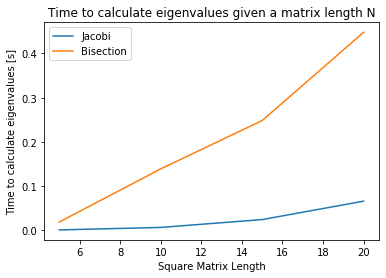
\includegraphics[scale=0.6]{figure3.png}
    \caption{Comparison between the runtimes of the Jacobian and the Bisection solution of a matrix M.}
    \label{fig:3}
\end{figure} \newline
This is even slower than the Jacobi method.
\newpage
We've now extended our program to also account for a potential $V(\rho)$, and we get:
\begin{figure}[ht!]
    \centering
    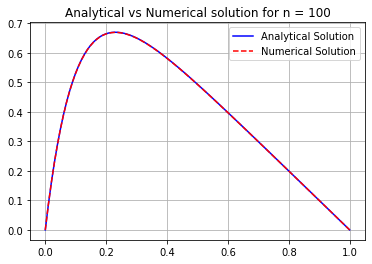
\includegraphics[scale=0.6]{figure5.png}
    \caption{Radial Solution as $\rho$ approaches a theoretical $\rho_{max}$ with 200 integration points.}
    \label{fig:4}
\end{figure}
In addition our program returns the following numerical eigenstates:
\begin{table}[ht!]
    \centering
    \begin{tabular}{c|c|c}
         & Numerical& Analytical&
         \lambda_1& 2.9992& 3& \\
         \lambda_2& 6.9961& 7&\\
         \lambda_3& 10.9905& 11&
    \end{tabular}
    \caption{Numerical eigenstates for N = 200}
    \label{tab:2}
\end{table}
\section{Discussion}
There's a couple of things I'd like to discuss regarding this project.
\paragraph{Analytical v. NumPy v. Jacobi.} \newline
For all three algorithms they deviated very little from each other. I see little reason to use the Jacobi function, especially when both C++ and Python has eig\textunderscore sym() and linalg.eig() respectively, especially with how flexible these are compared to the analytical solution, which only works for this matrix. Perhaps if I could further specialize the Jacobi Algorithm it would beat NumPy but I couldn't find any way to do that. \newpage
\paragraph{Eigenstates} \newline
Although the assignment specifically asked for 4 decimals precision, the runtime as $N$ increased was starting to become quite large, so I decided to stop at $N = 200$. This yielded quite accurate results, and I'd reckon an extra 50 to 100 would probably land us within the the 4 decimal precision mark. \newline
Had I used C++ (which I should, I'm just lazy), I would've probably been able to further optimize my program and made the runtime a lot more bearable. Additionally I've come across the python library pandas, which could've (to my knowledge) improved my runtimes, but I don't know the library well enough to justify using it, sadly.
\paragraph{Bisection} \newline
There's a few things I'd like to discuss regarding the bisection method I developed instead of solving 2e). Firstly, the most obvious point of discussion is it being slower than Jacobi's method, which I personally think shouldn't have been the case. \newline
I tried my best to follow the ALGOL code appended but I couldn't get it to work. I instead tried my own solution where I simply retrieved the characteristic polynomial using the SymPy library and bisected it to find it's roots, which are eigenvalues of the matrix. I think retrieving the characteristic polynomial is the primary reason for the slow calculation time, but I couldn't think of any other solution. 
\paragraph{Tests} \newline
For my tests, I decided to make a program that tests two different matrices' numerical eigenvalues up against their analytical ones for all three methods. \newline
This was simply done by declaring a matrix, and then running it through the three different algorithms to see if they were the same (within a tolerance). In this case we used a tridiagonal matrix on form \ref{eq:matrixse} where $n = 5, a = 2$ and $d = 5$. This should return the eigenvalues, $$\lambda = [7,5,3,5 + 2\sqrt(3), 5 - 2\sqrt(3)]$$
\begin{lstlisting}[language=Python]
rLambdas = np.sort([7,5,3,5 + 2*np.sqrt(3), 5 - 2*np.sqrt(3)])
A = tridiag(2,5,5)
"""
Let's now test each of our solutions
"""
nEigs = np.sort(np.linalg.eig(A)[0])
aEigs = np.sort(eigenvalues(2,5,5))
jEigs = np.sort(jacobi_solver(A)[0])
if np.allclose(rLambdas,nEigs) == True:
    print('Numpy Validated')
if np.allclose(rLambdas,nEigs) == True:
    print('Analytical Validated')
if np.allclose(rLambdas,nEigs) == True:
     print('Jacobi Validated')
\end{lstlisting} \newline
which it did, successfully. \newpage
Additionally we tested that our max\textunderscore sqr() function always returns the highest non-diagonal (the sub-diagonal, in our case).\newline We tried:
\begin{lstlisting}[language=Python]
def tridiagmod(a,d,n):
    A = np.zeros((n,n)) #n x n
    A[0][0] = d; A[0][1] = a
    k = 0
    for i in range(1,n):
        for j in range(3):
            if j == 0:
                A[i][j+k] = a+2*k-2
            elif j == 1:
                A[i][j+k] = d
            elif j ==2:
                if i != n-1:
                    A[i][j+k] = a+2*k
        k += 1
    return(A)
d = 5; a = 38; n = 5
A = tridiagmod(a,d,n)
x,y = max_sqr(A)
if A[x,y] == 42:
    print('max_sqr() Validated')
\end{lstlisting} \newline
This test was also a success, and we can conclude that our functions are working as intended.
\section{Conclusion}
In conclusion, we've shown four different methods of finding the eigenvalues (and eigenvectors) of a Toeplitz matrix. We've found that an analytical solution runs the fastest, as expected, but that though the Jacobi Algorithm works well for brute force, it is very slow comparatively to our other solutions, with the exception of the bisection method. We've also shown numerically the eigenstates of our one-dimensional one electron system to be $\lambda_1 = 3, \lambda_2 = 7, \lambda_3 = 11$ with a harmonic oscillator with the potential $V(\rho) = \rho^2$.
\bibliographystyle{unsrt}
\bibliography{citations.bib}
\end{document}
